\pdfoutput=1
\RequirePackage{amsmath}
\documentclass[iop, apj]{emulateapj}
%\usepackage[varg]{newtxmath}
%\usepackage{newtxtext}
\usepackage{txfonts}
\usepackage[spanish,es-minimal,english]{babel}
\usepackage[utf8]{inputenc}
\usepackage{natbib}
\usepackage{microtype}
\usepackage{hyperref}
\graphicspath{ {../original-papers/figs/}, {figs/}, {../}, {../luis-programas}}
\bibliographystyle{apj}


%% Commands for the postage stamp imagse
\setlength{\fboxsep}{0pt}%
\newlength\figwidth
\setlength\figwidth{0.32\textwidth}
\newlength\figstampcolsep
\setlength\figstampcolsep{5pt}
\newcommand\BowshockFig[1]{
  \includegraphics[width=\figwidth, clip, trim=60 50 100 50]
  {#1}
}
\newcommand\raiselabel[1]{\raisebox{0.5\figwidth}[-0.5\figwidth]{#1}}

\newcommand\oiii{[\ion{O}{3}]}
\newcommand\nii{[\ion{N}{2}]}
\newcommand\sii{[\ion{S}{2}]}
\newcommand\heii{[\ion{He}{2}]}
\newcommand\ha{\ensuremath{\mathrm{H\alpha}}}
\newcommand\hb{\ensuremath{\mathrm{H\beta}}}
\newcommand\hg{\ensuremath{\mathrm{H\gamma}}}
\newcommand\elec{\ensuremath{_{\mathrm{e}}}}
\newcommand\Te{\ensuremath{T\elec}}
\newcommand\Ne{\ensuremath{n\elec}}
\newcommand\Wav[1]{\ensuremath{\lambda #1}}
\newcommand\thC{\ensuremath{\theta^1\,\mathrm{Ori~C}}}

\renewcommand\clearpage{}

\begin{document}
\title{
  An Atlas of Stationary Bow Shock Arcs in the Orion Nebula
}
\author{
  William J. Henney, 
  Luis A. Gutiérrez-Soto,
  Jorge A. Tarango-Yong,
  Nahiely Flores-Fajardo
}

\affil{%
  \foreignlanguage{spanish}{Instituto de Radioastronomía y
    Astrofísica, Universidad Nacional Autónoma de México, Apartado
    Postal 3-72, 58090 Morelia, Michaoacán, Mexico};
  w.henney@crya.unam.mx, l.gutierrez@crya.unam.mx,
  j.tarango@crya.unam.mx}

\begin{abstract}
  We present a complete catalog of all the stationary emission line
  arcs (LL objects and proplyd bowshocks) found in archival HST imaging
  of the Orion Nebula.   The total number of objects detected is 73,
  of which 20 have not previously been reported in the literature.
  We classify the shapes of emission line arcs by fitting conic sections
  to the inner and outer shell boundaries and calculate the background
  corrected H alpha surface brightness of each object. We find significant
  differences in the shell shapes between the objects closest to the
  ionizing stars and those farther away.  The closer group, which all
  represent proplyd interactions with the hypersonic stellar wind,
  have relatively closed shapes, while the farther group, which are
  due to interactions with the transonic ionized champagne flow in
  the nebula, are more open and hyperbolic.  Although some of the
  latter group are also known proplyds, many are not, and the largest
  and brightest arcs tend to be associated with particularly luminous
  young stars, suggesting that the intrinsic T Tauri disk wind may play
  a role. The orientations of the arcs, together with the stagnation
  pressures estimated from the surface brightness, allow the internal
  velocity field of the H II region to be probed.  We find that
  approximately radial flows from the core of the nebula dominate over
  disordered, turbulent flows.
\end{abstract}

\section{Introduction}
\label{sec:intro}

\section{Observations}
\label{sec:observ}

\begin{deluxetable*}{l l l l l l}
  \tablecaption{Archival \textit{HST} imaging datasets used in this study
    \label{tab:programs}}  
  \tablehead{\colhead{Year} & \colhead{Instrument} & \colhead{Program(s)}
    & \colhead{Field size} & \colhead{Pixel size} & \colhead{Filters}}
  \startdata
  1994--5 & WFPC2/WFC & GTO~5085, GO~5469 & \(5' \times 10'\) & \(0.1''\)
  & F656N, F658N, F502N, F547M \\
  1994--5 & WFPC2/PC & GO~5469 & \(1' \times 2'\) & \(0.045''\)
  & F656N, F658N, F502N, F673N, F631N, F547M \\
  2004 & ACS/WFC & GO~9825 & \(20' \times 20'\) & \(0.05''\) & F658N \\
  2004--5 & ACS/WFC & GO~10246 & \(25' \times 30'\) & \(0.05''\) & F658N, F435W, F555W, F775W, F850LP \\
  2004--5 & WFPC2/WFC & GO~10246 & \(25' \times 30'\) & \(0.1''\) & F656N 
  \enddata
\end{deluxetable*}

We have attempted to identify and characterize all stationary
emission-line arcs in archival HST imaging observations of
the Orion Nebula, obtained with the WFPC2 and ACS cameras, as
summarized in Table~\ref{tab:programs}.  The primary dataset that
we have used is the 26-orbit Cycle~12 program GO~9825 \citep{Bally:2006a}.
This program covered a significant fraction of the entire nebula with
the ACS/WFC camera in the filter F658N, which transmits the lines
\ha{} \Wav{6563} and \nii{} \Wav{6584}.  The combination of good
spatial resolution and signal-to-noise of this dataset makes it ideal
for detecting the faint arcs against the varying nebular background.
For regions in the outskirts of the nebula that are outside of the
GO~9825 fields, we used observations with the same camera and filter
from the 104-orbit Cycle~13 program GO~10246 (\textit{HST} Treasury
Program on the Orion Nebula Cluster, \citealp{Robberto:2013a}).
In addition, we have used images from the same program obtained with
the F656N filter of the WFPC2 camera.  The resolution\footnote{The
point spread function is very similar for the two cameras
(FWHM \(\approx 0.082''\) at \ha{}), but it is not well-sampled by
the larger \(0.1''\) pixels of the three WFC chips of WFPC2.} and
signal-to-noise of these observations is significantly worse than
the ACS images, but they have the important advantage that the WFPC2
F656N filter is considerably narrower (\(\approx 5\)~\AA) than
the ACS F658N filter (\(\approx 15\)~\AA) and suffers relatively
little contamination from \nii{}.  Finally, for regions in the
core of the nebula, we have used older WFPC2 images from programs
GTO~5085 \citep{ODell:1996a} and GO~5469 \citep{Bally:1998a}.
These offer two advantages for the study of the bowshocks closest
to the Trapezium OB stars: shorter exposure times mean that the
bright stars are less saturated, and images were obtained in a much
wider range of emission line filters.  


\newcommand\Rc{\ensuremath{R_{\mathrm{c}}}}
\begin{figure*}
  \includegraphics[width=\linewidth]{radius-methodology}
  \caption{Methodology for determining geometric parameters of the arcs.}
  \label{fig:r0-rc-method}
\end{figure*}
For each arc, we trace by eye the inner and outer boundaries of
the emission line shell and mark along each edge using ``point''
regions with the SAOimage ds9 program\footnote{\url{http://ds9.si.edu}},
and in addition mark the position of the central star or proplyd
(hereafter, central source). These are shown in
Figure~\ref{fig:r0-rc-method} as yellow crosses, yellow pluses
and blue circle for the outer edge, inner edge, and proplyd,
respectively, for an illustrative case. We then fit circular arcs
to the points, determining the center and radius of curvature \(\Rc\)
of each edge. The fits are carried out with the aid of the python
library lmfit\footnote{\url{https://pypi.python.org/pypi/lmfit/}},
which implements a Levenberg--Marquardt curve-fitting algorithm.
The initial parameter estimates for each fit are obtained as follows.
First, the sky coordinates \((\alpha_i, \delta_i)\) of the edge points
are converted to polar coordinates with respect to the central source:
\((r_i, \theta_i)\), where \(\theta\) is a position angle
(degrees counterclockwise from north). After sorting the edge points
in \(\theta\), the smallest value of \(r_i\), together with its immediate
neighbors to either side are used to define a parabola in polar
coordinates, the root of whose derivative gives the point \((r_0, \theta_0)\)
of closest approach of the arc's edge to the central source.\footnote{This
technique will fail if the closest edge point does not have a neighbor
to one side, that is, if it is at one end of the traced edge.
Such a situation is occasionally found when the observed arc is very
asymmetric. In this case a parabola is fitted to all of the edge points
\((r_i, \theta_i)\) in order to determine \((r_0, \theta_0)\).}
The initial estimate for the position of the center of curvature
is taken to be the same distance from the central source as the point
of closest approach, but on the ``other side'' of the source: that is
at polar coordinates \((r_0, \theta_0 + 180^{\circ})\).  The sky coordinates
of this center of curvature \((\alpha_{\mathrm{c}}, \delta_{\mathrm{c}})\)
are the only two formal parameters of the circle fit since the circle
radius is estimated on the fly as the mean distance \(\langle\Rc\rangle\)
from  \((\alpha_{\mathrm{c}}, \delta_{\mathrm{c}})\) to the individual edge
points \((\alpha_i, \delta_i)\).   Only those edge points satisfying the
condition \(|\theta_j - \theta_0| \le 90^\circ\) are used in the fit.

\begin{figure*}
  \includegraphics[width=\linewidth]{ll-pos-image}
  \caption{Position of bow shock arcs.}
  \label{fig:pos-image}
\end{figure*}

\begin{figure*}
  \includegraphics[width=\linewidth]{ll-pos-image-zoom}
  \caption{Position of bow shock arcs. Zoomed area.}
  \label{fig:pos-image}
\end{figure*}

\begin{figure*}
  \centering
  \includegraphics[width=\linewidth]{arc-classify}
  \caption{Spatial distribution of the bowshock arcs and
                     classification into spatial groups.}
  \label{fig:size-v-distance}
\end{figure*}

\section{Catalog}
\label{sec:catalog}

\subsection{LV knot group}
\label{sec:lv-group}
\begin{deluxetable*}{rrrrrrrrrrrrr}
\tablecaption{Shell geometric parameters of lv knots}
\tablehead{\colhead{Object} & \colhead{RA} & \colhead{Dec} & \colhead{\(D\)} & \colhead{PA} & \colhead{\(R_\mathrm{out}\)} & \colhead{\(R_\mathrm{in}\)} & \colhead{\(R_\mathrm{c,out}\)} & \colhead{\(R_\mathrm{c,in}\)} & \colhead{\(h\)} & \colhead{PA\(\mathrm{_{out}}\)} & \colhead{PA\(\mathrm{_{in}}\)} & \colhead{Star ID}}
\startdata
158-323 & 05:35:15.83 & $-$05:23:22.5 & 8.34 & 90.1 & 1.85 & 1.64 & 2.92 & 2.35 & 0.21 & 114.8 & 120.0 & ACS 4260 \\
161-324 & 05:35:16.06 & $-$05:23:24.3 & 5.29 & 70.1 & 1.16 & 0.90 & 3.01 & 2.03 & 0.26 & 70.7 & 76.6 & ACS 4383 \\
163-317 & 05:35:16.28 & $-$05:23:16.6 & 6.11 & 164.8 & 2.32 & 1.93 & 4.90 & 4.44 & 0.40 & 148.6 & 145.5 & ACS 4427 \\
166-316 & 05:35:16.61 & $-$05:23:16.2 & 7.15 & 207.0 & 0.69 & 0.41 & 1.19 & 0.85 & 0.28 & 181.4 & 160.5 & ACS 4470 \\
167-317 & 05:35:16.74 & $-$05:23:16.5 & 7.97 & 220.9 & 1.96 & 1.25 & 3.29 & 2.05 & 0.71 & 178.1 & 165.4 & RSS 10079 \\
168-328 & 05:35:16.76 & $-$05:23:28.1 & 7.79 & 315.2 & 1.06 & 0.79 & 1.31 & 0.80 & 0.27 & 345.3 & 353.0 & ACS 4552 \\
168-326 & 05:35:16.84 & $-$05:23:26.3 & 7.71 & 299.5 & 0.95 & 0.74 & 3.04 & 3.01 & 0.20 & 314.5 & 328.1 & ACS 4537
\enddata
\end{deluxetable*}

\begin{figure*}
  \setlength\tabcolsep{\figstampcolsep}
  \begin{tabular}{l l l }
    \BowshockFig{LV5-PC_mosaic_f656-images} & \BowshockFig{161-324-Bally_01-images} & \BowshockFig{LV3-PC_mosaic_f547-images} \\
    \raiselabel{(\textit{a})} & \raiselabel{(\textit{b})} & \raiselabel{(\textit{c})} \\
    \BowshockFig{166-316-Bally_01-images} & \BowshockFig{LV2-PC_mosaic_f656-images} & \BowshockFig{168-328-Bally_01-images} \\
    \raiselabel{(\textit{d})} & \raiselabel{(\textit{e})} & \raiselabel{(\textit{f})} \\
    \BowshockFig{168-326-Bally_01-images} \\
    \raiselabel{(\textit{g})} \\
  \end{tabular}
  \caption{Stationary arc sources in the LV knots group.}
  \label{fig:stamps-LV}
\end{figure*}


The LV knot group is a six proplyds set that were discovered by
\citet{Laques:1979a}, located very close to the Trapezium and show
an isotropic distribution. There is a binary system in this group.
The emission arcs were identified after. In general, these arcs
are very weak, which makes it difficult to trace the edges of the
shells.

\textit{158-323 (LV5).} This was previously catalogued as a round
head with tail by \citet{ODell:1996a}. After, it was reported
as a proplyd and binary system by \citep{Ricci:2008a}. An emission
arc wraps around this proplyd. 
 
\textit{161-324 (LV4).} This small and bright proplyd was
previously catalogued by \citet{ODell:1996a, Ricci:2008a}. The
proplyd is surrounded by a faint but well-defined emission arc.
It is located about \(4.0''\) to the southeast of 158-323.

\textit{163-317 (LV3).} This proplyd previously catalogued by
\citet{ODell:1996a, Ricci:2008a} is surrounded by a faint and
small emission arc. 

\textit{166-316. (LV2b)} This was reported as a circularly symetric
source by \citet{ODell:1996a}. Later, this source was catalogued as
a proplyd by \citet{Ricci:2008a}. 

\textit{167-317 (LV2).} This bright proplyd was previously catalogued
by \citet{ODell:1994a, Ricci:2008a}. It exhibits a long tail. An
obvious emission arc \citep{Bally:2000a} wraps around the proplyd.
\citet{Bally:2000a} describe a compact microjet emerging from this
proplyd. 

\textit{168-328.} This small proplyd was previously reported
by \citet{ODell:1994a} and \citet{Ricci:2008a}. An emission arc is
associated with this proplyd. The arc is much fainter than the
proplyd. This object is located about \(2.1''\) to the southwest
of LV1.  

\textit{168-326 (LV1).} This is a previously reported proplyd
designated 168-326S \citep{ODell:1994a}. This proplyd was classified
as a binary system by \citet{Ricci:2008a}. An arc emision with a
complex morphology is surrounded this proplyd.


\clearpage
\subsection{Southeast group}
\label{sec:se-group}
\begin{deluxetable*}{rrrrrrrrrrrr}
\tablecaption{Shell geometric parameters of southeast group}
\tablehead{\colhead{Object} & \colhead{RA} & \colhead{Dec} & \colhead{\(D\)} & \colhead{PA} & \colhead{\(R_\mathrm{out}\)} & \colhead{\(R_\mathrm{in}\)} & \colhead{\(R_\mathrm{c,out}\)} & \colhead{\(R_\mathrm{c,in}\)} & \colhead{\(h\)} & \colhead{PA\(\mathrm{_{out}}\)} & \colhead{PA\(\mathrm{_{in}}\)}}
\startdata
169-338 & 05:35:16.88 & $-$05:23:38.0 & 17.14 & 334.7 & 1.03 & 0.68 & 2.04 & 0.72 & 0.35 & 345.9 & 6.4 \\
177-341 & 05:35:17.67 & $-$05:23:41.0 & 26.54 & 314.0 & 3.81 & 3.06 & 4.25 & 3.87 & 0.75 & 317.0 & 293.7 \\
180-331 & 05:35:18.03 & $-$05:23:30.8 & 25.91 & 288.7 & 1.44 & 1.11 & 2.36 & 1.77 & 0.33 & 280.8 & 282.0 \\
189-329 & 05:35:18.87 & $-$05:23:28.9 & 37.56 & 279.7 & 1.40 & 0.54 & 6.32 & 0.83 & 0.86 & 296.4 & 264.0
\enddata
\end{deluxetable*}

\begin{figure*}
  \setlength\tabcolsep{\figstampcolsep}
  \begin{tabular}{l l l }
    \BowshockFig{169-338-Bally_01-images} & \BowshockFig{177-341-Bally_01-images} & \BowshockFig{180-331-Bally_01-images} \\
    \raiselabel{(\textit{a})} & \raiselabel{(\textit{b})} & \raiselabel{(\textit{c})} \\
    \BowshockFig{189-329-Bally_01-images} \\
    \raiselabel{(\textit{d})} \\
  \end{tabular}
  \caption{Stationary arc sources in the Southeast group.}
  \label{fig:stamps-SE}
\end{figure*}


The southeast group is located to the inside of the Orion Nebula.
The central sources of their members are proplyds and their LL arcs
associated have not been previously reported in the literature.
Their diffuse shells are very thin. 

\textit{169-338.} This is a small and faint previously reported
proplyd \citep{ODell:1994a, Ricci:2008a} with a well defined tail.
The emission arc associated to this proplyd is very faint and clumpy
but well-defined. 

\textit{177-341 (HST 1).} This very large proplyd with a long tail was
previously catologed by \citet{ODell:1994a, Ricci:2008a}. There is
probably a jet that emerges from the proplyd \citep{Bally:2000a}.
We identified a well-defined but faint  emission arc associated with
this proplyd.

\textit{180-331.} This was first cataloged as a star by
\citet{ODell:1996a}. Later, this was reported as a proplyd and a
binary system by \citet{Ricci:2008a}. The proplyd is surrounded by
a highly asymmetric emission arc.

\textit{189-329.}  The central source was first classified as star
by \citet{ODell:1996a} and later as a proplyd by \citet{Ricci:2008a}.
This object is a very faint proplyd associated with a very diffuse
shell. The northern bow wing is much more extended than the southern
wing. The fact that the shell is so large and diffuse, may be an
indication that it is not related to the proplyd, although the fact
that a small cavity is seen  around the proplyd suggests that some
degree of physical interaction is indeed occurring.


\clearpage
\subsection{North group}
\label{sec:n-group}
\begin{deluxetable*}{rrrrrrrrrrrrrrr}
\tablecaption{Shell geometric parameters of north group}
\tablehead{\colhead{Object} & \colhead{RA} & \colhead{Dec} & \colhead{\(D\)} & \colhead{PA} & \colhead{\(R_\mathrm{out}\)} & \colhead{\(R_\mathrm{in}\)} & \colhead{\(\Pi_\mathrm{out}\)} & \colhead{\(\Pi_\mathrm{in}\)} & \colhead{\(\Lambda_\mathrm{out}\)} & \colhead{\(\Lambda_\mathrm{in}\)} & \colhead{\(h\)} & \colhead{PA\(\mathrm{_{out}}\)} & \colhead{PA\(\mathrm{_{in}}\)} & \colhead{Star ID}}
\startdata
154-240 & 05:35:15.38 & $-$05:22:39.8 & 45.30 & 160.6 & 2.48 & 1.72 &  & 2.09 &  & 1.38 & 0.40 & 132.6 & 196.4 & ACS 4112 \\
170-249 & 05:35:16.97 & $-$05:22:48.4 & 35.16 & 194.2 & 3.23 & 2.45 & 1.61 & 1.28 &  &  & 0.78 & 173.4 & 193.3 & ACS 4586
\enddata
\end{deluxetable*}

\begin{figure*}
  \setlength\tabcolsep{\figstampcolsep}
  \begin{tabular}{l l l }
    \BowshockFig{142-301-Bally_01-images} & \BowshockFig{154-225-Bally_01-images} & \BowshockFig{154-240-Bally_01-images} \\
    \raiselabel{(\textit{a})} & \raiselabel{(\textit{b})} & \raiselabel{(\textit{c})} \\
    \BowshockFig{159-221-Bally_01-images} & \BowshockFig{163-222-Bally_01-images} & \BowshockFig{165-235-Bally_01-images} \\
    \raiselabel{(\textit{d})} & \raiselabel{(\textit{e})} & \raiselabel{(\textit{f})} \\
    \BowshockFig{170-249-Bally_01-images} & \BowshockFig{178-258-Bally_01-images} \\
    \raiselabel{(\textit{g})} & \raiselabel{(\textit{h})} \\
  \end{tabular}
  \caption{Stationary arc sources in the North group.}
  \label{fig:stamps-N}
\end{figure*}


The north group is located inside of the orion Nebula.

\textit{142-301.} The central source was first catalogued as
cusp with tail \citep{ODell:1996a} and later as proplyd
\citep{Bally:2000a, Ricci:2008a}. This large proplyd has
one of the longest tails (\(4''\)) of any proplyd and does
not have a hemispherical head. Instead, the ionization front
appears to trace the disk surface, which is inclined with
respect to the tail by about $55^{\circ}$. The proplyd tail
points away from \(\mathrm{\theta^1\,Ori~A}\) instead of \thC~and
exhibits some bends and wiggles \citep{Bally:2000a}. This proplyd
is surrounded by a very faint emission arc.  Rather than showing
continuous curvature, the emission arc appears to comprise two
straight edges, which meet at a point south-east of the proplyd,
with the shell being thicker on the southern side.

\textit{154-225.} The central source was previously catalogued
as elongated body with diffuse boundary \citep{ODell:1996a}.
Later, \citet{Ricci:2008a} reported it as proplyd in a binary
sytem (the main body). The central source is sorrounded by a
very faint and lumpy emission arc.

\textit{154-240.} The central source is a large bright
proplyd \cite{Bally:2000a, Ricci:2008a} with a \(3''\)
long tail and the inclined protoplanetary disk is seen
in silhouette \citep{Bally:2000a}. There is evidence of
an emission arc associated with this proplyd, but only
the inner edge can be clearly traced. The outer edge of
the shell merges with a thick knotty structure whose origin
is unclear.

\textit{159-221.} This central source was first classified as
a star by \citet{ODell:1996a}. This same source was reported as
a dark disk seen only in silhouette by \citet{Ricci:2008a}.
But a faint emission rim can be seen surrounding the disk in
the \ha{} image, suggesting that it is an externally ionized
proplyd. We identified an emission arc associated with the
central star. The outer edge of the shell is very diffuse,
which  makes it difficult to trace of outer rim. The axis of
the bowshock is significantly deviates from the radial
direction.

\textit{163-222.} The central proplyd was first catalogued
by \citet{ODell:1996a}. There is a compact \(0.''15\) diameter
disk seen nearly in face-on embedded in this stubby
proplyd \citep{Bally:2000a, Ricci:2008a}.  This source
was also reported as a binary sytem \citep{Ricci:2008a}.
An a very faint and small emission arc wraps the proplyd.
The outer and inner edges of the shell are well-defined on
the eastern side, nevertheless the western side is superimposed
on an unrelated a brighter larger scale emission filament,
making impossible to trace the arc boundaries on this side.

\textit{165-235.} This was previously catalogued as a star
by \citet{ODell:1996a}. Later, It was classified as proplyd
by \citet{Ricci:2008a}. This proplyd is sorrounde by a
previously uncatalogued emission arc. This emission arc is
very faint.


\textit{170-249.} This central source is a previously
catalogued proplyd \citep{ODell:1996a}, reported as a
binary system by \citet{Ricci:2008a}. This bright and
large proplyd exhibits a long tail and an inclined disk
seen in silhouette \citep{Bally:2000a}. Several
filamentary emission features with arc shape crosses the
object, nonetheless it is possible to identify a very faint
emission arc that seems to be associated to the proplyd.  

\textit{178-258.}  This large and weak proplyd was catalogued
by \citet{Ricci:2008a}, which is surrounded by a well-defined
but faint emission arc.

\clearpage
\subsection{Northwest group}
\label{sec:nw-group}
\begin{deluxetable*}{rrrrrrrrrrrrrrr}
\tablecaption{Shell geometric parameters of northwest group}
\tablehead{\colhead{Object} & \colhead{RA} & \colhead{Dec} & \colhead{\(D\)} & \colhead{PA} & \colhead{\(R_\mathrm{out}\)} & \colhead{\(R_\mathrm{in}\)} & \colhead{\(\Pi_\mathrm{out}\)} & \colhead{\(\Pi_\mathrm{in}\)} & \colhead{\(\Lambda_\mathrm{out}\)} & \colhead{\(\Lambda_\mathrm{in}\)} & \colhead{\(h\)} & \colhead{PA\(\mathrm{_{out}}\)} & \colhead{PA\(\mathrm{_{in}}\)} & \colhead{Star ID}}
\startdata
049-143 & 05:35:04.94 & $-$05:21:42.9 & 197.82 & 120.2 & 1.17 & 0.62 & 2.63 & 1.06 &  & 1.10 & 0.56 & 103.1 & 139.0 & ACS 2608 \\
051-024 & 05:35:05.13 & $-$05:20:24.3 & 245.01 & 136.7 & 1.19 & 0.90 & 1.83 & 1.65 & 1.77 & 2.14 & 0.27 & 136.5 & 123.6 & ACS 2628 \\
072-134 & 05:35:07.20 & $-$05:21:34.3 & 174.74 & 128.3 & 4.69 & 2.26 & 2.81 & 2.80 & 2.10 & 2.50 & 2.42 & 89.7 & 94.5 & ACS 2840 \\
w073-227 & 05:35:07.27 & $-$05:22:26.5 & 147.27 & 112.4 & 1.63 & 0.81 & 2.41 & 3.41 & 2.86 & 3.31 & 0.70 & 117.0 & 120.5 & ACS 2842 \\
074-229 & 05:35:07.38 & $-$05:22:28.9 & 144.78 & 111.7 & 1.36 & 0.79 & 1.15 &  &  &  & 0.60 & 120.3 & 185.7 & ACS 2854 \\
101-233 & 05:35:10.13 & $-$05:22:32.6 & 105.94 & 118.1 & 2.46 & 2.11 & 2.25 & 1.95 &  &  & 0.42 & 131.4 & 136.6 & ACS 3172 \\
102-157 & 05:35:10.25 & $-$05:21:57.1 & 125.30 & 133.0 & 0.80 & 0.40 & 8.14 & 4.22 & 3.17 & 2.56 & 0.45 & 118.5 & 116.6 & ACS 3192 \\
106-245 & 05:35:10.58 & $-$05:22:44.7 & 94.70 & 113.5 & 0.63 & 0.23 & 2.99 & 3.27 & 2.54 & 2.69 & 0.38 & 122.7 & 99.0 & ACS 3241 \\
109-246 & 05:35:10.90 & $-$05:22:46.3 & 89.68 & 113.8 & 1.95 & 1.32 & 6.73 & 10.33 & 3.08 & 3.11 & 0.70 & 112.9 & 119.5 & ACS 3294 \\
124-131 & 05:35:12.38 & $-$05:21:31.4 & 126.20 & 151.7 & 4.48 & 2.74 &  &  &  &  & 1.73 & 134.9 & 156.0 & ACS 3497 \\
206-043 & 05:35:20.56 & $-$05:20:43.1 & 171.16 & 201.3 & 1.61 & 1.12 & 1.33 & 1.91 &  &  & 0.44 & 176.1 & 182.7 & ACS 5514
\enddata
\end{deluxetable*}

\begin{figure*}
  \setlength\tabcolsep{\figstampcolsep}
  \begin{tabular}{l l l }
    \BowshockFig{049-143-Bally_09-images} & \BowshockFig{051-024-Bally_09-images} & \BowshockFig{072-134-Bally_09-images} \\
    \raiselabel{(\textit{a})} & \raiselabel{(\textit{b})} & \raiselabel{(\textit{c})} \\
    \BowshockFig{w073-227-Bally_01-images} & \BowshockFig{074-229-Bally_01-images} & \BowshockFig{101-233-Bally_01-images} \\
    \raiselabel{(\textit{d})} & \raiselabel{(\textit{e})} & \raiselabel{(\textit{f})} \\
    \BowshockFig{102-157-Bally_01-images} & \BowshockFig{106-245-Bally_01-images} & \BowshockFig{109-246-Bally_01-images} \\
    \raiselabel{(\textit{g})} & \raiselabel{(\textit{h})} & \raiselabel{(\textit{i})} \\
    \BowshockFig{206-043-Bally_02-images} \\
    \raiselabel{(\textit{j})} \\
  \end{tabular}
  \caption{Stationary arc sources in the Northwest group.}
  \label{fig:stamps-NW}
\end{figure*}


The bowshock northwest group is located to the outskirt of
the Orion Nebula. The mostly the emission arcs this group
have been reported in the literature, with the exception
of the  073-227 arc, which it was already previously reported.    

\textit{4578-251.} This is a very bright T Tauri star
associated with an emission arc that presents a double-shell
morphology. This object has an asymmetric bow shock and
the shell is more extended toward the south than to the north.
The emission of the outer shell is fainter than the inner
shell and is unclear whether the region marked with points
is part of the outer shell.

\textit{049-143.} Figure shows a proplyd \citep{Ricci:2008a}
with a very diffuse arc of emission. Its shell is thick,
the wings of the bow shock are very open, and circular
shaped. The inner edge is more diffuse than the outer edge
and the bow shock is asymmetric. The  proplyd has a short
tail, probably indicating that it is highly inclined and
there is extinction in the center. 
 
\textit{051-024.} We identified a previously uncataloged
proplyd with its bow shock located in front of the upper
end of the North Bright Bar. The emission shell is thin,
but a second larger, and more diffuse, emission shell is
seen in front of the bow shock that we have
marked. It is unclear whether this outer shell is related
to the object or not. If it is, then the object would be
similar to the nearby 072-134. 

\textit{072-134.} This object is located to the southeast
from 051-134. It was first cataloged by \citet{ODell:1996a}
and designated as 072-135. Later, \citet{Ricci:2008a} listed
it as disk seen nearly edge-on, named 072-135. In this work
a shell with a complex morphology is identified. The inner
edge is a narrow bright arc, while the shell is thick and
faint, which is only visible on the N~side.                 

\textit{073-227.} \citet{Bally:2000a} reported a wind
collision front associated with 073-227. The well-defined
outer edge of the arc deviates significantly from the
circular fit in the south wing of the bowshock.
   
\textit{074-229.} This central source is located at south
east of 073-227. It is a T Tauri star, that appears to be
the smaller twin of the nearby 073-227, associated with a
small and faint emission bow shock. The central star is
not obviously a proplyd, but this may be because it is too
small to be resolved. The projected separation from 072-134
is about \(8''.0\), which is not significantly smaller than
the expected mean projected separation between nearest
neighbors given the stellar density at this distance from
the Trapezium \citep{Reipurth:2007a}, 
% http://adsabs.harvard.edu/abs/2007AJ....134.2272R
so the evidence that they form a physical binary pair is weak.

\textit{101-233.} The central source was first cataloged
as proplyd by \citet{ODell:1996a}, designated as 102-233,
and later by \citet{Ricci:2008a} with the same name. This
proplyd is associated with a clumpy, thin and low ionization
bow shock. Several additional broad filamentary emission
features can be seen in front of the arc, but it is unclear
if these are associated with the object or are a chance
superposition, that also seem to be aimed toward Trapezium. 

\textit{102-157.} We identified a previously uncataloged
proplyd associated with a very faint emission arc. The proplyd
tail is very short, indicating that it is highly inclined.
102-157 has a open bow. The southwest wing of the bowshock
is crossed by an apparently unrelated east-west oriented
filament, which makes it difficult to trace the emission
arc on this side.


\textit{106-245 and 109-246.} The bright proplyd 109-246
\citep{Ricci:2008a} was previously cataloged as 109-247 by
\citet{Bally:2000a}, who noted its central dark disk and
possible microjet.  The proplyd is situated just outside
the HH~202 bow shock and is superimposed on a complex
background of fainter HH bow shocks that point towards
the north west.  However, a south-east facing bow shock
is also clearly visible just in front of
the proplyd.  We identify this as a stationary arc due to its
symmetric placement with respect to the proplyd axis and clear
morphological differences from the HH bow shocks.

A similar, albeit much smaller arc can be seen in front of the
stellar source 106-245.  Given the complex nebular background,
the evidence for an arc is not overwhelming, but is strengthened
by the morphological similarity with the nearby 109-246.  As
with 074-249, the source is not obviously a proplyd, but again
this may be simply due to its small size.  


\textit{124-131.} This object is a circumbinary proplyd, that was
first cataloged by \citet{ODell:1996a}, but they named it 124-132 and
classified as irregular. Later, this source was reported by
\citet{Smith:2005a} showing a microjet emerging perpendicular to the
major axis of the disk. \citet{Ricci:2008a} cataloged the source as a
binary system and \citet{Robberto:2008a} interpreted the central dark
silhouette as a circumbinary disk.  We report the discovery of a
broad, faint partial shell in front of the proplyd, which we identify
as a stationary arc.  The arc is barely visible in \ha{}, but is much
clearer in green and blue wideband filters, suggesting that we are
seeing dust-scattered continuum.  In this respect it is similar to the
arc in front of the close-in proplyd 163-317 (LV~3).   


\textit{132-053.}  Similar area to 131-046, and also may be affected
by extinction filaments.  The shell looks more convincing in this
object however, particularly the innner edge.


\textit{206-043.} This object appears to show an extremely faint
emission arc.  However, it is seen against a strongly variable nebula
background and a filamentary foreground extinction feature is seen
nearby (\(\approx 3''\) to west).  It is therefore possible that
the apparent arc is merely an ilusion caused by an extension of these
extinction filaments.  Although it is not cataloged as a proplyd, the
central source shows indications of a faint conical tail, pointing
almost due North, with a length \(\approx 2''\). 

\clearpage
\subsection{Southwest group}
\label{sec:sw-group}
\input{table-sort-05-southwest.tex}
\input{fig-stamps-05-southwest.tex}

\newcommand\Ricci{R08}
\newcommand\Bally{BOM00}
\newcommand\ODell{OW96}

\begin{deluxetable*}{l ll lp{0.3\linewidth}}
  \tablecaption{Notes on Southwest Group}
  
  \tablehead{\colhead{Source} & \colhead{Proplyd} & \colhead{Star}
    & \colhead{Arc} & \colhead{Notes}}
  \startdata
  4582-635 & \Ricci{} & \nodata & New & Very faint \\
  000-400 & \Ricci{} & \nodata & \Bally{} & Designated 4596-400 in \Ricci{} \\
  005-514 & \ODell{} & \nodata & \Bally{} & \\
  012-407 & No & \nodata & \Bally{} & Thick, diffuse arc\\ 
  014-414 & No & \nodata & \Bally{} & Double central star \\
  022-635 & No & \nodata & New & Asymmetric arc\\
  030-524 & ? & \nodata & \Bally{} & Flat, asymmetric arc, apparent
  proplyd tail \\
  \enddata
\end{deluxetable*}

The bowshock southwest group is located to the outskirts of the
Orion Nebula. The mostly of its members are the tipycal LL Ory arcs,
with its well-defined emission arc.  

\textit{4582-635.} This is a previously cataloged proplyd
\citep{Ricci:2008a}, which is surrounded by a very faint emission arc
that has not been reported previously in the literature. There are
hints of additional emission knots in front of the arc, but the S/N is
very low and it is unclear if they are related with the object.

\textit{4596-400.} \citet{Bally:2000a} first reported this object as a
``wind collision front'' with the designation 000-400. The central
source was identified as a proplyd by \citet{Ricci:2008a}, who gave it
the designation 4596-400 based on more accurate astrometry, which we
adopt here. The outer edge of the wings of the emission arc can be
traced to much farther distances than is typical, at least 5 times the
axial radius of curvature. The northern wing appears knotty at large
distances, whereas the southern wing is smooth. However, the knots
seen superimposed on the northern wing may be due to an unrelated,
larger scale filament that crosses both this object and 012-407, which
is most prominent in blue/green continuum filters.

\textit{000-400.} \citet{Bally:2000a} reported a wind collision fronts
associated with w000-400. The central source is a previously catalogued
proplyd, designated 4596-400 \citep{Ricci:2008a}. The outer edge of
the wings of the emission arc can be traced to much farther distances
than is typical, at least 5 times the axial radius of curvature.
The northern wing becomes knotty at large distances, where  the southern
wing is smoothes. The bow shock has parabolic morphology and wraps around
a proplyd (Fig.).   

\textit{005-514.} This proplyd was first cataloged by \citet{ODell:1996a}.
Later, \citet{Bally:2000a} reported a fainter and smaller wind-wind
collission front, designated w005-514 and was show in \ha{} image.
The lower (southeast) wing of the arc has a complex structure, with
multiple overlapping filaments.

\textit{012-407.} \citet{Bally:2000a} reported a wind collision fronts
associated with 012-407. The bright central star is not obviously a
proplyd. The diffuse shell is very thick.  

\textit{014-414.} \citet{Bally:2000a} cataloged another wind collision
front associated with 014-407. It is one of the smaller LL arcs in this
group, containing a double central star. A larger scale filament which
is prominent in blue/green continuum crosses the object, but seems to be
unrelated. 

\textit{022-635.} This is a previously uncataloged arc of emission that
wraps around a T Tauri star. The north wing of the bowshock is more
extended than south wing. There are two apparently unrelated emission
filaments that cross this object. 

\textit{030-524.} \citet{Bally:2000a} reported a wind-wind collision front,
associated with w030-524. The central source has a tail oriented away from
the Trapezium, indicating a proplyd. The northern outer edge of the
asymmetric shell is very flat and it makes a sharp corner where it joins
the head of the shell.

\textit{041-637.} This is a previously reported star \citep{Da-Rio:2009a}
associated with a faint emission arc. There is a west faint emission arc,
which is probably unrelated to the object. The emission arc has not been
previously reported in the literature.

\textit{042-628.} This source appears in the proplyd catalog of
\citet{Ricci:2008a} with the designation 038-627, supposedly based on
appearance in previous catalogs \citep{ODell:1996a}. However, we haver
been unable to locate the source in any other catalogs and the source
coordinates clearly indicate a designation of 042-628, which we adopt
here.  A bright compact knot is seen just inside the emission arc,
\(\approx 2''\) to the north of the proplyd, which may represent a
jet.  A fainter knot is also seen closer to the proplyd, but at a
slightly larger position angle.

\textit{044-527.} A faint and small emission arc associated with 044-527
was cataloged by \citet{Bally:2000a}. The central source was subsequently
classified as proplyd by \citet{Ricci:2008a}. This object has a jet
parallel to the proplyd axis. The bowshock is very asymmetric.

\textit{LL 1 (056-519).} The T Tauri star LL Orionis is the prototype
of the LL objects. Its emission arc was discovered by
\citet{Gull:1979a} and is now denoted LL 1. This is a parabolic or
hyperbolic bowshock that wraps around the source star
\citep{Bally:2006a}. This emission arc was also reported by
\citet{Bally:2000a} and as a LL Orionis-type wind-wind collision
fronts LL 1 by \citet{Bally:2001a}. The emission of the bowshock wings
is blueshifted with repect to the backgraond nebular emission, the
emission from the head of the bowshock is at a similar velocity to the
nebula and shows no detectable proper motion, consistent with it being
a stationary structure \citep{Henney:2013a}. LL 1 is associated with a
hypersonic jet Herbig-Haro, HH 888, that arises in the T Tauri star.
    

\textit{069-601.} This was first classified as a non-proplyd stellar
source by \citet{ODell:1996a}. Later, a wind collision front was
reported by \citet{Bally:2000a} associated with w069-601.
\citet{Ricci:2008a} catalogued the central source as a proplyd.
The parabolic arc emission is well-defined, which makes it easy to
trace the edges of the shell. The arc shape is very similar to LL 1,
but is considerably smaller. 

\clearpage
\subsection{West group}
\label{sec:w-group}
\begin{deluxetable*}{rrrrrrrrrrrrr}
\tablecaption{Shell geometric parameters of west group}
\tablehead{\colhead{Object} & \colhead{RA} & \colhead{Dec} & \colhead{\(D\)} & \colhead{PA} & \colhead{\(R_\mathrm{out}\)} & \colhead{\(R_\mathrm{in}\)} & \colhead{\(R_\mathrm{c,out}\)} & \colhead{\(R_\mathrm{c,in}\)} & \colhead{\(h\)} & \colhead{PA\(\mathrm{_{out}}\)} & \colhead{PA\(\mathrm{_{in}}\)} & \colhead{Star id}}
\startdata
4285-458 & 05:34:28.52 & $-$05:24:57.9 & 721.18 & 82.4 & 1.91 &  & 4.34 &  & \nodata & 87.0 &  & V* V976 Ori \\
LL3 & 05:34:40.81 & $-$05:26:38.5 & 566.33 & 69.8 & 3.12 & 1.28 & 6.54 & 3.08 & 1.83 & 89.2 & 99.6 & V* V2005 Ori \\
LL2 & 05:34:40.86 & $-$05:22:42.2 & 532.12 & 94.3 & 4.04 & 2.07 & 27.93 & 13.84 & 1.13 & 97.6 & 89.5 & V* IX Ori \\
4417-653 & 05:34:41.70 & $-$05:26:52.9 & 559.12 & 67.9 & 1.19 & 0.72 & 2.90 & 1.67 & 0.45 & 57.3 & 49.8 & V* V399 Ori \\
LL4 & 05:34:42.72 & $-$05:28:37.2 & 593.11 & 58.0 & 2.42 & 1.42 & 11.79 & 4.95 & 0.99 & 46.7 & 40.3 & V* V2012 Ori \\
4468-605 & 05:34:46.76 & $-$05:26:04.8 & 471.30 & 69.9 & 2.47 & 1.33 & 7.11 & 2.22 & 1.20 & 54.2 & 59.6 & V* V2026 Ori \\
4491-627 & 05:34:49.07 & $-$05:26:26.5 & 447.58 & 65.7 & 2.02 & 1.19 & 4.17 & 2.45 & 0.79 & 72.3 & 76.4 & V* V2044 Ori \\
4505-336 & 05:34:50.49 & $-$05:23:35.3 & 386.95 & 88.1 & 1.62 & 0.93 & 3.49 & 1.98 & 0.66 & 99.8 & 99.5 & V* V475 Ori \\
4520-419 & 05:34:52.01 & $-$05:24:18.7 & 368.41 & 81.2 & 1.39 & 1.07 & 2.92 & 2.30 & 0.32 & 84.3 & 85.2 & V* V2064 Ori \\
4531-628 & 05:34:53.07 & $-$05:26:27.6 & 394.31 & 62.0 & 0.79 & 0.46 & 1.52 & 0.93 & 0.33 & 104.0 & 89.0 & 2MASS J05345307-0526276 \\
4550-659 & 05:34:55.01 & $-$05:26:58.8 & 385.57 & 55.9 & 1.61 & 0.88 & 3.82 & 2.23 & 0.45 & 68.1 & 71.8 & V* V2074 Ori \\
4578-251 & 05:34:57.79 & $-$05:22:51.1 & 279.49 & 96.5 & 1.85 & 1.19 & 3.52 & 2.07 & 0.53 & 81.2 & 125.0 & V* V402 Ori \\
4582-635 & 05:34:58.17 & $-$05:26:35.1 & 333.37 & 54.7 & 1.11 & 0.68 & 2.93 & 2.06 & 0.46 & 65.7 & 50.5 & 2MASS J05345816-0526350 \\
w000-400 & 05:34:59.57 & $-$05:24:00.1 & 254.03 & 81.5 & 1.47 & 0.80 & 4.37 & 2.43 & 0.68 & 71.9 & 73.4 & V* V1318 Ori \\
w005-514 & 05:35:00.47 & $-$05:25:14.3 & 262.72 & 64.8 & 1.65 & 1.20 & 3.45 & 2.03 & 0.44 & 64.5 & 57.9 & V* V2102 Ori \\
w012-407 & 05:35:01.17 & $-$05:24:06.7 & 231.47 & 79.0 & 2.29 & 0.95 & 6.74 & 4.26 & 1.23 & 68.3 & 69.7 & Brun 471 \\
w014-414 & 05:35:01.37 & $-$05:24:13.4 & 229.95 & 77.2 & 1.21 & 0.37 & 2.19 & 1.61 & 0.70 & 98.3 & 93.2 & [OW94] 014-413 \\
022-635 & 05:35:02.20 & $-$05:26:35.3 & 286.47 & 47.7 & 1.10 & 0.75 & 4.46 & 2.29 & 0.34 & 83.2 & 77.5 & [H97b] 10351 \\
w030-524 & 05:35:03.00 & $-$05:25:24.4 & 234.09 & 58.6 & 0.63 & 0.29 & 2.56 & 1.54 & 0.32 & 93.8 & 82.0 & [LRT2005] 030-524 \\
041-637 & 05:35:04.06 & $-$05:26:37.1 & 267.84 & 43.4 & 1.94 & 1.19 & 4.39 & 3.23 & 0.77 & 4.2 & 15.5 & V* V1482 Ori \\
042-628 & 05:35:04.20 & $-$05:26:27.6 & 259.59 & 44.5 & 3.07 & 1.76 & 6.90 & 3.61 & 1.34 & 61.6 & 56.1 & V* V1322 Ori \\
w044-527 & 05:35:04.43 & $-$05:25:27.4 & 217.94 & 55.0 & 2.13 & 0.78 & 3.25 & 1.53 & 0.85 & 121.2 & 267.4 &  \\
LL1 & 05:35:05.64 & $-$05:25:19.4 & 198.63 & 53.9 & 3.06 & 1.90 & 8.72 & 7.13 & 1.13 & 84.4 & 78.1 & V* LL Ori \\
w069-601 & 05:35:06.91 & $-$05:26:00.6 & 212.19 & 41.9 & 0.85 & 0.41 & 2.72 & 1.77 & 0.42 & 86.1 & 87.1 & V* V2170 Ori
\enddata
\end{deluxetable*}

\begin{figure*}
  \setlength\tabcolsep{\figstampcolsep}
  \begin{tabular}{l l l }
    \BowshockFig{4285-458-Robberto_ACS_1r_f658n-images} & \BowshockFig{LL3-Bally_17-images} & \BowshockFig{LL2-Bally_18-images} \\
    \raiselabel{(\textit{a})} & \raiselabel{(\textit{b})} & \raiselabel{(\textit{c})} \\
    \BowshockFig{4417-653-Bally_17-images} & \BowshockFig{LL4-Bally_24-images} & \BowshockFig{4468-605-Bally_17-images} \\
    \raiselabel{(\textit{d})} & \raiselabel{(\textit{e})} & \raiselabel{(\textit{f})} \\
    \BowshockFig{4491-627-Bally_17-images} & \BowshockFig{4505-336-Bally_17-images} & \BowshockFig{4520-419-Bally_17-images} \\
    \raiselabel{(\textit{g})} & \raiselabel{(\textit{h})} & \raiselabel{(\textit{i})} \\
    \BowshockFig{4531-628-Bally_16-images} & \BowshockFig{4550-659-Bally_16-images} & \BowshockFig{4578-251-Bally_09-images} \\
    \raiselabel{(\textit{j})} & \raiselabel{(\textit{k})} & \raiselabel{(\textit{l})} \\
  \end{tabular}
  \caption{Stationary arc sources in the West group.}
  \label{fig:stamps-W}
\end{figure*}


This sparsely populated group is located in the outskirts of the Orion
Nebula. 

\textit{4285-458.} This is an emission arc that wraps a bright T~Tauri
star. Although the outer boundary of the shell is well-defined, it is
impossible to trace the shell's inner boundary due to confusion with
the PSF wings of the central star. This is the most distant emission
arc from the Trapezium in this catalog and It is also much smaller
than the other arcs in the west group.

\textit{LL 3 (4408-639).} This previously reported LL~Ori-type object
\citep{Bally:2001a} exhibits a double-shell morphology to the emission
arc: an inner shell that is brighter and narrower, and an outer shell
that is fainter and broader, but still with a well-defined outer edge.
In addition, the central star shows a faint emission structure, which
protrudes to the WSW, and which may represent a proplyd tail, although
the object is not included in any proplyd catalogs, such as
\citet{Ricci:2008a}.

\textit{LL 2 (4409-242).} This large LL~Ori-type object
\citep{Bally:2001a}, is associated with the T~Tauri star IX~Ori. It
also has a bipolar jet, HH~505, which is oriented nearly perpendicular
to the bowshock axis. Apart from LL~1, this is the only LL object
whose kinematics have been studied via spectroscopic mapping
\citep{Henney:2013a}. Unlike LL~1, the structure and kinematics of the
LL~2 arc are very asymmetrical.  Additionally, proper motion studies
\citep{Henney:2013a} show that only the head and northern wing of the
arc are stationary structures: the southern portion of the arc has
high proper motion and seems to be driven by the blueshifted jet.

\textit{LL 4 (4427-838).} This is a previously reported LL~Ori-type
object \citep{Bally:2001a}. The central source was reported as a
proplyd and a binary system by \citet{Bally:2006a}. At first glance,
this object appears to be a single arc with a very large radius of
curvature. However wide closer inspection suggests that the ``wings''
of the arc are separate structures from the more curved nose
region. We suggest that they may not be part of the true LL arc, but
are instead driven by the bipolar jet \citep{Bally:2006a} in a similar
way to the southern wing of LL~2.

\textit{4468-605.}  This arc was first reported by \citet{Bally:2006a}
who also noted the proplyd nature of the central source and the
presence of a microjet (HH 886) oriented approximately parallel to the
symmetry axis of the proplyd and arc.  Although \citet{Bally:2006a}
report the jet as one-sided, a bright \ha{} filament seen at the end
of the proplyd tail may represent the counterjet.  The north side of
the emission arc shows an apparent flared morphology, but this may be
illusory, due to an unrelated larger scale emission filament that is
projected against that side of the bowshock.

\clearpage
\subsection{South group}
\label{sec:s-group}
\begin{deluxetable*}{rrrrrrrrrrrrrrr}
\tablecaption{Shell geometric parameters of south group}
\tablehead{\colhead{Object} & \colhead{RA} & \colhead{Dec} & \colhead{\(D\)} & \colhead{PA} & \colhead{\(R_\mathrm{out}\)} & \colhead{\(R_\mathrm{in}\)} & \colhead{\(\Pi_\mathrm{out}\)} & \colhead{\(\Pi_\mathrm{in}\)} & \colhead{\(\Lambda_\mathrm{out}\)} & \colhead{\(\Lambda_\mathrm{in}\)} & \colhead{\(h\)} & \colhead{PA\(\mathrm{_{out}}\)} & \colhead{PA\(\mathrm{_{in}}\)} & \colhead{Star ID}}
\startdata
066-3251 & 05:35:06.57 & $-$05:32:51.4 & 587.49 & 14.5 & 1.07 &  & 1.49 &  & 1.19 &  &  & 300.1 &  & ACS 2787 \\
116-3101 & 05:35:11.65 & $-$05:31:01.0 & 463.92 & 8.8 & 1.45 & 1.00 & 1.57 & 1.88 & 1.55 & 1.69 & 0.44 & 24.0 & 7.9 & ACS 3390 \\
119-3155 & 05:35:11.93 & $-$05:31:53.3 & 515.10 & 7.4 & 3.02 & 1.95 & 1.70 & 2.65 & 1.62 & 2.04 & 1.00 & 33.3 & 35.3 & ACS 3438 \\
136-3057 & 05:35:13.61 & $-$05:30:57.6 & 456.93 & 5.2 & 10.13 & 4.91 & 1.80 & 5.98 & 1.78 & 2.39 & 4.51 & 10.9 & 4.4 & ACS 3764 \\
138-3024 & 05:35:13.80 & $-$05:30:24.4 & 423.64 & 5.2 & 3.89 & 2.74 & 1.96 & 1.66 &  & 1.62 & 1.11 & 22.2 & 17.4 & ACS 3756 \\
203-3039 & 05:35:20.29 & $-$05:30:39.4 & 440.72 & 352.4 & 5.38 & 1.76 & 3.14 & 7.03 & 2.38 & 3.83 & 3.06 & 359.4 & 8.2 & ACS 5456 \\
261-3018 & 05:35:26.17 & $-$05:30:18.0 & 440.40 & 340.6 & 4.99 & 2.51 & 7.35 & 1.55 & 4.02 & 3.33 & 2.59 & 1.7 & 357.1 & ACS 6473 \\
w266-558 & 05:35:26.62 & $-$05:25:58.3 & 218.16 & 315.6 & 1.88 & 1.13 & 5.42 & 1.32 & 2.16 & 2.07 & 0.78 & 330.7 & 298.5 & ACS 6559 \\
305-811 & 05:35:30.44 & $-$05:28:11.2 & 356.86 & 324.0 & 1.72 & 0.89 & 3.63 & 6.57 &  &  & 0.80 & 358.6 & 349.7 & ACS 7023 \\
308-3036 & 05:35:30.79 & $-$05:30:36.3 & 484.13 & 333.6 & 2.56 & 1.44 & 1.61 & 1.09 & 1.62 & 1.08 & 1.12 & 359.9 & 329.8 & ACS 7074 \\
LL5 & 05:35:31.40 & $-$05:28:16.4 & 369.54 & 322.7 & 2.96 & 1.46 & 2.26 & 2.23 & 2.81 & 1.98 & 1.49 & 339.7 & 339.7 & ACS 7161 \\
LL6 & 05:35:32.87 & $-$05:30:21.5 & 485.82 & 329.6 & 3.63 & 1.63 & 6.01 & 4.90 & 3.72 & 4.17 & 2.05 & 7.6 & 18.0 & ACS 7338 \\
344-3020 & 05:35:34.36 & $-$05:30:20.6 & 496.76 & 327.3 & 1.66 & 0.67 & 2.17 & 4.82 & 2.23 & 2.45 & 0.95 & 334.9 & 325.5 & ACS 7458 \\
LL7 & 05:35:35.13 & $-$05:33:49.2 & 686.23 & 335.9 & 7.00 & 5.53 &  &  &  &  & 1.46 & 359.2 & 3.8 & ACS 7547 \\
362-3137 & 05:35:36.35 & $-$05:31:37.8 & 577.96 & 329.0 & 3.12 & 1.57 & 1.32 & 1.41 &  & 1.10 & 1.47 & 6.4 & 267.8 & ACS 7661 \\
364-411 & 05:35:36.44 & $-$05:34:11.1 & 714.33 & 335.2 & 3.04 &  &  &  &  &  &  & 341.1 &  & ACS 7676
\enddata
\end{deluxetable*}

\begin{figure*}
  \setlength\tabcolsep{\figstampcolsep}
  \begin{tabular}{l l l }
    \BowshockFig{116-3101-Bally_14-images} & \BowshockFig{119-3155-Bally_14-images} & \BowshockFig{136-3057-Bally_14-images} \\
    \raiselabel{(\textit{a})} & \raiselabel{(\textit{b})} & \raiselabel{(\textit{c})} \\
    \BowshockFig{203-3039-Bally_14-images} & \BowshockFig{261-3018-Bally_07-images} & \BowshockFig{w266-558-Bally_06-images} \\
    \raiselabel{(\textit{d})} & \raiselabel{(\textit{e})} & \raiselabel{(\textit{f})} \\
    \BowshockFig{308-3036-Bally_08-images} & \BowshockFig{LL5-Bally_07-images} & \BowshockFig{LL6-Bally_08-images} \\
    \raiselabel{(\textit{g})} & \raiselabel{(\textit{h})} & \raiselabel{(\textit{i})} \\
    \BowshockFig{344-3020-Bally_08-images} & \BowshockFig{LL7-Robberto_ACS_7l_f658n-images} & \BowshockFig{362-3137-Bally_08-images} \\
    \raiselabel{(\textit{j})} & \raiselabel{(\textit{k})} & \raiselabel{(\textit{l})} \\
    \BowshockFig{364-411-Robberto_ACS_7l_f658n-images} \\
    \raiselabel{(\textit{m})} \\
  \end{tabular}
  \caption{Stationary arc sources in the South group.}
  \label{fig:stamps-S}
\end{figure*}


The bowshock south group is located in the outskirts of the Orion
Nebula and southeast of the Bright Bar, several members of this
group are the farthest objects from the Trapezium. The objects
are generally large in this group and many have a bright inner rim.   

\textit{066-3251.} This object was classified as a proplyd
by \citet{Ricci:2008a} and, located at a distance \(\sim 10'\)
south of the ONC core, it is one of the farthest known proplyds
from the Trapezium. We have identified a faint arc associated
with this proplyd, which is seen most clearly in the F555W broad
band filter but is also visible in the \ha{} filter. This object
is projected onto the tip of a large-scale wishing bone shaped
filament, which seems to represent a local ionization front.
We believe that the ``outflow'', which \citet{Ricci:2008a} identify
to the south of this object is merely a misidentification of
part of this filament.  

\textit{116-3101.} Figure shows a proplyd associated with a small
but sharply defined emission arc.  The central star is also
named V488 Ori \citep{Bally:2006a}. The wings of the bow shock
are very closed, the outer edge is well defined and has a circular
shape since we can fit a perfect circle with the points marked.  

\textit{119-3155.} This is a binary system associated with an
emission arc. Based on the position of the outer of curvature of
the arc, we assign the fainter, more northern binary component as
the corresponding stellar source. It has a faint arc to the north
and another to the east (Fig), but  the east arc is probably
unrelated to the object, and may instead be associated with the
HH 880 bowshock which passes \(15''\) to the south. This emission
arc has not been previously reported in the literature.     

\textit{136-3057.} This is a T Tauri star associated with an
emission arc. It is located to the north of 119-3155 and is
one of the bigger objects of this group. 136-3057 has a very
diffuse shell. This has not been previously reported in the
literature.

\textit{138-3024.} Figure shows a T Tauri star associated with a
thin shell. The arc is seen most strongly blue and green broad
band filters, but it is also seen at very low contrast in the \ha{}
filter. This object has not been previously reported in the
literature.

\textit{203-3039.} This object has a microjet (HH 561) which was
discovered in the Fabry-Pérot study of the southern Orion Nebula
by \citet{Bally:2001a}. Later, this HH object was described in
more detail by \citet{Bally:2006a}, the microjet emerges toward
the east from the variable star MY Ori, terminating in a faint
bowshock at a distance of \(16''\). A fainter counterjet and
bowshock are located west of the star. In addition to these
previously reported features, we identify an LL-type emission arc
associated with MY Ori. The faint bow is very open.

\textit{261-3018.} This is a relatively large and diffuse LL-type
arc previously unreported, seen superimposed on a very complicated
region of overlapping flows. We tentatively identify the star 261-3018
as the source, although the star (264-3016) is another possible
candidate. In the \ha{} the 261-3018 star (which is the same source
as 262-3018 reported by \citealp{Bally:2006a})  shows a linear protrusion
of length \(\simeq1''\) towards the southwest. This is unlikely to be
a proplyd tail, since it is not aligned with the radial direction from
the Trapezium, and instead may be a microjet. Indeed, a series of faint
knots and bowshocks extend for \(30''\) in the same direction.
The LL-type arc is very flat and shows a bright rim at its inner edge.
It extends further to the east than to the west. The object is seen
in projection superimposed on the HH 502 flow but shows no evidence
of physical interaction with this flow.

\textit{266-558.} \citet{Bally:2000a} catalogued a wind collision
front associated with w266-558. Figure shows emission shell that
wraps around the source. The source is a previously catalogued
proplyd by \citet{Ricci:2008a}. w266-558 presents a double-shell
morphology, with knotty bow wings. The bow wings are very open.
Although, we have assigned this object to the south group, it is
located much closer to the Trapezium than the other members, in
a region lacking in other arcs.

\textit{305-811.} Previously classified as LL-type object
by \citet{Bally:2006a}. The emission arc is extremely faint
and asymmetric. The star shows  a faint protrusion to the
southeast in the \ha{} filter, probably indicating a proplyd
tail, although the source has not previously been catalogued as
a proplyd.    

\textit{308-3036.} \citet{Bally:2006a} reported a bright star,
that is surrounded by a faint arc of emission, located to the west
of LL 6. This object has a nearly circular inner shock, the circle
fit is roughly centered on the star. The circular silhouette
(see Fig.) may trace a wind cavity, or possibly a dusty envelope
surrounding the star \citep{Bally:2006a}.       

\textit{LL 5 (315-816).} This is a LL Ori type object identified in
the outskirts of the Orion Nebula, it was first reported by
\citet{Bally:2001a}. Later, it was also catalogued by
\citet{Bally:2006a} and they mentioned that LL 5 is associated
with the  V1559 Ori star. This object has a short jet (HH 875
\citealp{Bally:2006a}) emerging from the proplyd toward the northeast.
The emission arc wraps around a proplyd, and was designated LLP 315-816
or 314-816. This object has a double-shell morphology with a bright
inner rim.
       
\textit{LL 6 (329-3021).} \citep{Bally:2001a} identified a LL Orionis-type
wind-wind collision fronts LL 6 in the outskirts of the Orion Nebula. LL 6
is associated with the star NX Ori, which is surrounded by a large arc of
emission \citep{Bally:2006a}. The wings of the bowshock are very open and
extended. This object has a prominent, one-sided jet, oriented perpendicular
to the axis of the LL arc. It is difficult to distinguish between the wings
of the LL arc and the jet-driven bowshocks.    

\textit{344-3020.} \citet{Bally:2006a} catalogued a proplyd associated
with an emission arc, designated as LL 344-3020. This object is very faint
and has a bipolar jet at P.A. = $45^{\circ}$.     

\textit{LL 7 (351-3349).} This object is a LL-type bowshock previously
reported by \citet{Bally:2001a}. The central source is a previously
catalogued proplyd \citep{Ricci:2008a}, designated 351-3349. This object
has a jet at P.A. $\sim 80^{\circ}$ perpendicular to LL arc axis. The
bowshock wings are very open, and it is one of the most distant emission
arcs from the Trapezium in this catalog. This object is larger than we show,
the bowshock from jet overlap wings of LL arc (see \citealp{Bally:2001a}).   

\textit{362-3137.} This is a previously uncatalogued proplyd associated with
an emission arc. However, \citet{Da-Rio:2009a} catalogued the central source
as a star. The source is a double star. It is located at north of LL 7.
This object seems to show a double-shell morphology. There is a filament
to south probably unrelated to the object. This emission arc has not been
previously reported in the literature.  

\clearpage
\subsection{Interproplyd shells}
\label{sec:interproplyd-group}
\begin{deluxetable*}{rrrrrrrrrrrrrrr}
\tablecaption{Shell geometric parameters of interproplyd shells}
\tablehead{\colhead{Object} & \colhead{RA} & \colhead{Dec} & \colhead{\(D\)} & \colhead{PA} & \colhead{\(R_\mathrm{out}\)} & \colhead{\(R_\mathrm{in}\)} & \colhead{\(\Pi_\mathrm{out}\)} & \colhead{\(\Pi_\mathrm{in}\)} & \colhead{\(\Lambda_\mathrm{out}\)} & \colhead{\(\Lambda_\mathrm{in}\)} & \colhead{\(h\)} & \colhead{PA\(\mathrm{_{out}}\)} & \colhead{PA\(\mathrm{_{in}}\)} & \colhead{Star ID}}
\startdata
160-350 & 05:35:15.96 & $-$05:23:49.7 & 27.91 & 13.3 & 0.11 & 0.04 &  &  &  &  & 0.07 & 226.2 & 224.3 & ACS 4341 \\
162-456 & 05:35:16.18 & $-$05:24:56.4 & 93.91 & 1.9 & 0.29 & 0.21 &  &  &  &  & 0.09 & 28.8 & 49.2 & ACS 4351 \\
168-326N & 05:35:16.83 & $-$05:23:26.0 & 7.49 & 297.4 & 0.23 & 0.12 & 5.82 & 6.26 &  & 3.36 & 0.11 & 137.0 & 142.2 & ACS 4567 \\
173-342 & 05:35:17.32 & $-$05:23:41.4 & 23.46 & 323.5 & 1.29 & 0.83 & 2.95 & 2.46 &  &  & 0.46 & 82.2 & 76.1 & ACS 4671 \\
204-330 & 05:35:20.40 & $-$05:23:30.0 & 60.39 & 277.1 & 0.33 & 0.11 & 3.87 & 7.42 &  & 2.01 & 0.22 & 112.4 & 119.0 & ACS 5475
\enddata
\end{deluxetable*}

\begin{figure*}
  \setlength\tabcolsep{\figstampcolsep}
  \begin{tabular}{l l l }
    \BowshockFig{160-350-PC_mosaic_f502-images} & \BowshockFig{162-456-Robberto_ACS_0l_f658n-images} & \BowshockFig{168-326N-Bally_01-images} \\
    \raiselabel{(\textit{a})} & \raiselabel{(\textit{b})} & \raiselabel{(\textit{c})} \\
    \BowshockFig{173-342-Bally_01-images} & \BowshockFig{204-330-Bally_06-images} \\
    \raiselabel{(\textit{d})} & \raiselabel{(\textit{e})} \\
  \end{tabular}
  \caption{Stationary arc sources in the Interproplyd shells.}
  \label{fig:stamps-*I}
\end{figure*}


The interproplyd shell is a  group of small proplyds, which they are
associated with small emission arcs which are formed by the interactions
between two individual photoevaporation flows.
    
\textit{160-350.} This was previously reported as an irregular proplyd
by \citet{Odell:1994} and was designated 159-350. Later, \citet{Ricci:2008a}
cataloged it as a binary system and ionized disk seen in emission.
The 159-350 outflow interact with the 160-350 flow producing a small
emission arc.  

\textit{162-456.} \citet{ODell:1996a} cataloged this object as a stellar
source and designated it 162-457. It was listed as a pre-main-sequence
binary star by \citet{Reipurth:2007}. A small emission arc is formed by
the interaction of the flows come from 162-456 and 162-456NE, the latter
located in the Northeast of 162-456.     

\textit{168-326N.} This source was previously reported as an unclear object
due to saturation by \citet{Odell:1994}. Later, it was catalogued as a proplyd
and binary system by \citet{Ricci:2008a}. Comparing the 5 GHz radio emission
to the \ha{} and \oiii{} $\lambda$5007 emission is perceptive a radio source
between southeast radio source 168-326SE and the northwest radio source
168-326NW. This structure is probably an interacting zone between the two
components \citep{Graham:2002}. From Fig. ?? in not possible to see
any emission arc because the system is very affected by saturation.    

\textit{173-342.} This was classified as a semi-stellar and elongated
object with diffuse boundary and appears designated 173-341 \citet{Odell:1994}.
This source was identified as a proplyd and binary system by \citet{Ricci:2008a}.
The emission arc is probably formed by the interaction of 173-342 with
177-341 (HST1). The arc emission shock in clearly visible in the image. 

\textit{175-321.} This was catalogued as a stellar source by \citet{ODell:1996a}.
The emission arc is not produced by the interaction of two proplyd flows. However,
the shock seems to be oriented towards th1D, which is very close to it. This arc
has not been reported in the literature.

\textit{204-330.} This source was previously reported as a proplyd and binary
system by \citet{Ricci:2008a} on which appears with the designation 204-330.
Due to the interaction between the flows of 204-330 and 205-330 proplyds is
formed small and faint emission arc. This shock has also not been reported
in the literature.

\clearpage
\subsection{New arc discoveries}
\label{sec:new}

\textit{4417-653.} This is a star previously catalogued by \citet{Hillenbrand:1997}.
There is an emission arc associated with this source. The shock has not been
reported in the literature. This object is located 20 arcsec to the southeast
of LL 3. The arcs have very open wings.  

\textit{4491-627.} This is a pre-main-sequence star catalogued by
\citet{Parihar:2009}. The shock associated with this source has not been
listed previously. It is a small and faint arc.

\textit{4550-659.} This source was previously catalogued as a pre-main-sequence
star by \citet{Parihar:2009}. The arc associated with this star has not been
reported in the literature. It is a large arc with very open wings. It seems
that two jets arise in the stellar component. A bright jet to the northwest
and a smaller one to the southeast of the star.  

\textit{4531-628.} This object is a pre-main-sequence star \citep{Da-Rio:2009a}
which has associated an emission arc that has not been previously reported.
It is a very small and faint arc.

\textit{4520-419.} The stellar component was previously reported
by \citet{Parihar:2009}. This pre-main-sequence star might be a proplyd
because it appears to have a small tail. The associated arc has not been
reported in the literature. It is a very weak arc with a circular and
symmetric shape. 

\textit{4505-336.} The star associated with the shock was catalogued
by \citet{Hillenbrand:1997}. The arc has not been reported in the
literature. The north wing of the arc is not visible. A very faint jet
seems to go north of the star. It probably ends in a bow shock.    

\textit{364-411.} The star was catalogued by \citet{Hillenbrand:1997}.
The arc associated to this star has not been reported. The outer
arc only can be traced, because the inner one can not be seen.
It is located approximately 25 arcsec to the southeast of LL 7.
Making of it the most distant arcs from the Trapezium. 

\clearpage
\subsection{Ambiguous objects}
\label{sec:problematic-objects}

\textit{065-502.} This was classified as a non-proplyd stellar source
by \citet{ODell:1996a}. However, the star has a small protrusion
pointing away from Trapezium, which may indicate a proplyd tail. This
proplyd tail is very short, suggesting that the object it is highly
inclined.  A very faint and diffuse arc can be discerned in front of
the object, but it is superimposed on an irregular background, which
makes it difficult to delineate its form.

\textit{066-652.}  This is in the distant south of the nebula and is
so faint that it is impossible to tell whether the nebulosity
associated with the star is a stationary arc or instead a
bright-rimmed globule. 

\textit{083-435.} The central source shows a very faint tail
suggesting that this source is a previously uncatalogued proplyd.
There is slight evidence for a broad diffuse emission arc in front
of the proplyd, but the source is near to the ``SW Cloud'' foreground
extinction feature \citep{ODell:2000a}, and the presence of faint
extinction filaments complicates the identification.


\textit{117-421.} This small proplyd \citep{Ricci:2008a} appears to
excavate a small cavity around it, but no shell outer edge is
evident.  Additionally, as for 083-435, the proximity to foreground
extinction filaments may be a confusing factor. 

\textit{121-434.}  Another small proplyd in the same area, with the
appearance of a clump emission arc in front of it.  However, once
again, the highly variable extinction makes the identification
uncertain. 

\textit{131-046.}  There is the appearance of a very broad and flat
shell in front of this proplyd.  However, it is in a region that is
Cross-crossed by multiple extinction filaments and the apparent shell
may be an illusion. 


\textit{173-236.} This large proplyd is has the weak evidence for an
emission arc in front of it, but it has a very small radius of
curvature compared with the other arcs.  It is located near to the
``Dark Bay'' \citep{ODell:2000a} and is crossed by multiple extinction
filaments, which make the identification uncertain.

\textit{212-400.}  A small proplyd with weak evidence for an emission
arc in front of it.  As with 173-236, it is near to the ``Dark Bay''
and the apparent arc may be an illusion caused by inhomogeneous
foreground extinction.

\textit{244-440.} Giant proplyd.  Seems to be in a cavity with a
well-defined inner border.  But it is not concave around the proplyd.
May be a larger scale feature related to the Bright Bar or to
HH~203/204.

\textit{266-500 (approx).} Proplyd. Evidence for small concave arc.
This might go in a new group of th1A objects.

\textit{095-800 (approx).} Very bright star with reflection nebula
and cometary shaped arc. 

\label{sec:problematic-group}
\begin{deluxetable*}{rrrrrrrrrrrrr}
\tablecaption{Shell geometric parameters of problematic objects}
\tablehead{\colhead{Object} & \colhead{RA} & \colhead{Dec} & \colhead{\(D\)} & \colhead{PA} & \colhead{\(R_\mathrm{out}\)} & \colhead{\(R_\mathrm{in}\)} & \colhead{\(R_\mathrm{c,out}\)} & \colhead{\(R_\mathrm{c,in}\)} & \colhead{\(h\)} & \colhead{PA\(\mathrm{_{out}}\)} & \colhead{PA\(\mathrm{_{in}}\)} & \colhead{Star ID}}
\startdata
065-502 & 05:35:06.54 & $-$05:25:01.5 & 177.29 & 56.1 & 1.42 & 0.49 & 7.74 & 2.31 & 1.21 & 90.5 & 104.7 & ACS 2783 \\
083-435 & 05:35:08.29 & $-$05:24:34.9 & 140.89 & 59.1 & 1.25 & 0.54 & 2.00 & 0.66 & 0.58 & 84.0 & 40.5 & ACS 2951 \\
117-421 & 05:35:11.65 & $-$05:24:21.4 & 92.07 & 50.2 & 2.00 & 0.71 & 6.95 & 2.77 & 1.37 & 99.1 & 96.7 & ACS 3388 \\
121-434 & 05:35:12.12 & $-$05:24:33.8 & 95.58 & 41.8 & 0.76 & 0.34 & 1.41 & 0.69 & 0.39 & 65.4 & 66.2 & ACS 3463 \\
131-046 & 05:35:13.06 & $-$05:20:45.8 & 164.46 & 162.4 & 3.55 & 1.00 & 7.33 & 5.64 & 2.17 & 140.3 & 144.2 & ACS 3586 \\
132-053 & 05:35:13.20 & $-$05:20:52.6 & 157.31 & 162.4 & 0.72 & 0.32 & 1.80 & 0.68 & 0.39 & 153.9 & 167.0 & ACS 3618 \\
173-236 & 05:35:17.35 & $-$05:22:35.7 & 48.96 & 197.1 & 2.28 & 1.53 & 1.36 & 1.94 & 0.75 & 255.3 & 275.5 & ACS 4705 \\
175-321 & 05:35:17.46 & $-$05:23:21.1 & 16.03 & 264.7 & 2.03 & 1.38 & 2.48 & 2.63 & 0.60 & 298.7 & 324.5 & ACS 4719 \\
212-400 & 05:35:21.18 & $-$05:24:00.5 & 80.99 & 297.9 & 1.07 & 0.84 & 0.83 & 0.52 & 0.21 & 331.2 & 335.5 & ACS 5617
\enddata
\end{deluxetable*}

\begin{figure*}
  \setlength\tabcolsep{\figstampcolsep}
  \begin{tabular}{l l l }
    \BowshockFig{065-502-Bally_01-images} & \BowshockFig{083-435-Bally_01-images} & \BowshockFig{117-421-Bally_01-images} \\
    \raiselabel{(\textit{a})} & \raiselabel{(\textit{b})} & \raiselabel{(\textit{c})} \\
    \BowshockFig{121-434-Bally_01-images} & \BowshockFig{131-046-Bally_02-images} & \BowshockFig{132-053-Bally_02-images} \\
    \raiselabel{(\textit{d})} & \raiselabel{(\textit{e})} & \raiselabel{(\textit{f})} \\
    \BowshockFig{173-236-Bally_01-images} & \BowshockFig{175-321-Bally_01-images} & \BowshockFig{212-400-Bally_06-images} \\
    \raiselabel{(\textit{g})} & \raiselabel{(\textit{h})} & \raiselabel{(\textit{i})} \\
  \end{tabular}
  \caption{Stationary arc sources in the Problematic objects.}
  \label{fig:stamps-*P}
\end{figure*}


\label{sec:notshell}



\clearpage
\section{Discussion}
\label{sec:discuss}
\begin{figure}
  (\textit{a})\\
  \includegraphics[width=\linewidth]{proplyd-star-ratio}\\
  (\textit{b})\\
  \includegraphics[width=\linewidth]{bowshock-proplyd-ratio}
  \caption{(\textit{a})~Fraction of all optically visible stars that
    are proplyds (dark circle symbols) or have bowshocks (light square
    symbols) as a function of projected separation from the Trapezium.
    (\textit{b})~Ratio between number of bowshocks and number of
    proplyds as a function of projected separation from the Trapezium.
    Dark circle symbols show all bowshocks in our catalog (with the
    exception of interproplyd shocks) while light square symbols show
    only those bowshocks associated with known or suspected proplyds.
  }
  \label{fig:bow-proplyd-star-ratios}
\end{figure}

Proplyd over star fraction falls off relatively smoothly with
projected distance.  Albeit with a sudden drop after about
200 arcsec.


Bowshock over proplyd fraction seems to have three separate peaks.
Very small distances corresponding to the wind-wind interaction,
then there is a dearth of bowshocks until a second peak around
four arcmin.  Finally at very large radii there may be a third
peak of objects that are not proplyds.

But an alternate explanation for the third peak could be that
they are all proplyds but that the proplyd fraction is
underestimated at large distances.

On the other hand there is also evidence for three distinct
populations from the azimuthal distribution around the Trapezium.
The group at 4 arcmin separation are mainly to the west whereas
the more distant objects are mainly to the south.


\begin{figure}
  \centering
  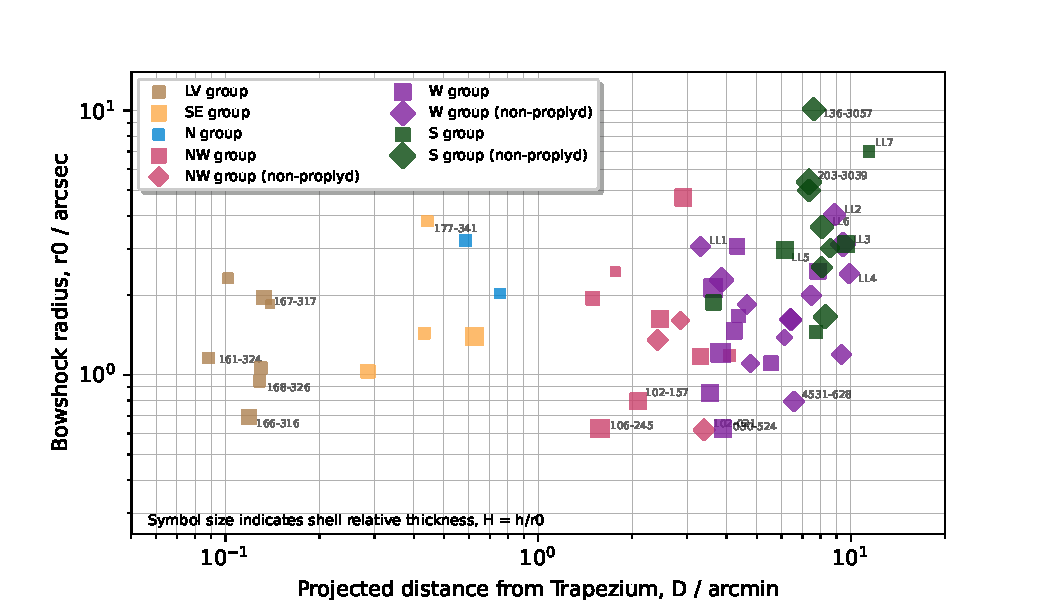
\includegraphics[width=\linewidth]{will-r0-vs-D-class}
  \caption{Bowshock axial size versus distance from the Trapezium.}
  \label{fig:size-v-distance}
\end{figure}
\begin{figure}
  \centering
  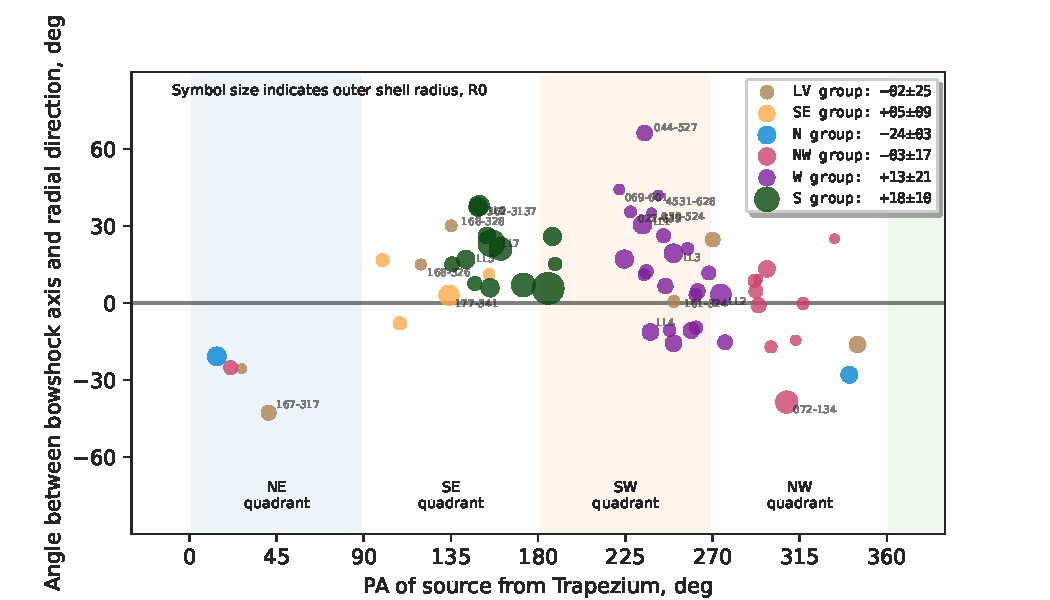
\includegraphics[width=\linewidth]{will-PA-vs-PA-class}
  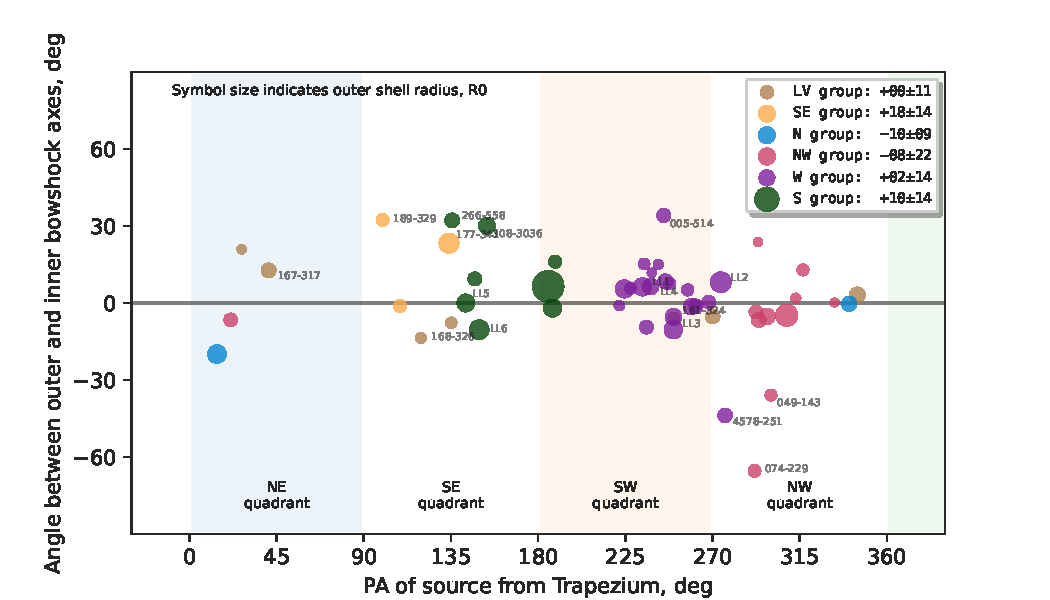
\includegraphics[width=\linewidth]{will-PA-out-vs-in-class}
  \caption{Angle offset between bowshock axis and the radial direction to \thC{}.}
  \label{fig:PA-v-PA}
\end{figure}
\begin{figure}
  \centering
  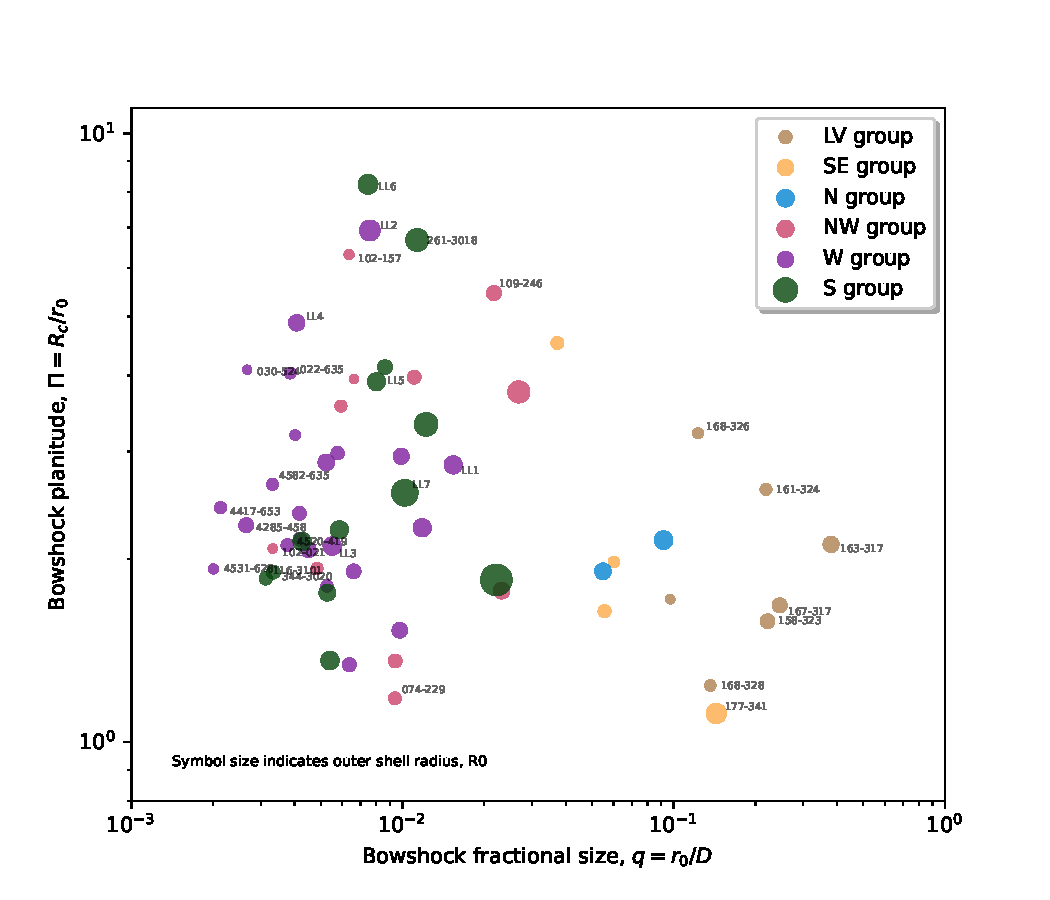
\includegraphics[width=\linewidth]{will-A-vs-q-class}
  \caption{Bowshock bluntness versus relative size.}
  \label{fig:A-v-q}
\end{figure}
\begin{figure}
  \centering
  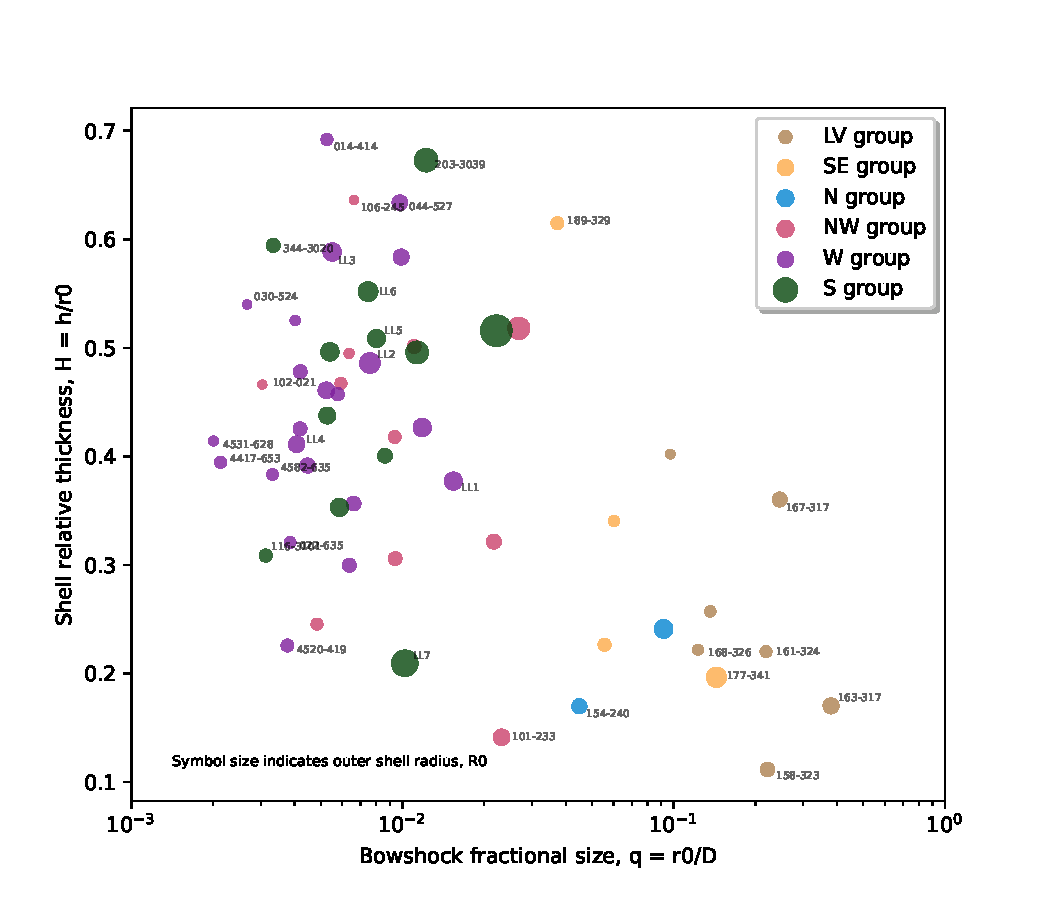
\includegraphics[width=\linewidth]{will-H-vs-q-class}
  \caption{Bowshock relative shell thickness versus relative size.}
  \label{fig:PA-v-PA}
\end{figure}

\begin{figure}
  \centering
  \includegraphics[width=\linewidth]{spiral-bars}
  \caption{The interlocking spirals.}
  \label{fig:spiral-bars}
\end{figure}

\begin{figure*}
  \centering
  \includegraphics[width=\linewidth]{orion-3d-twin-view}
  \caption{Simplified three-dimensional structure of the Orion Nebula.}
  \label{fig:3d-twin}
\end{figure*}

For clarity, we have omitted many secondary features and slightly
increased the size of the smaller features, such as Orion~South. 
The sizes of the smaller features  of the different features have been
modified slightly

\bibliography{ll-refs}


\end{document}

%%% Local Variables:
%%% mode: latex
%%% TeX-master: t
%%% End:
